\documentclass[prd,twocolumn,nofootinbib,superscriptaddress,amsmath,amssymb]{revtex4-2}
% Journal target not fixed (PRD vs EPJC): switch class later.
\usepackage{graphicx}
\usepackage{hyperref}

\begin{document}

\title{Decaying charged quirks: terminating non-helical tracks from SU(2)-multiplet quirks at the LHC}

\author{Amine Alida}
\affiliation{Laboratory of Material and Subatomic Physics, Faculty of Sciences, Ibn Tofail University, Kenitra, Morocco}

\begin{abstract}
TODO (write last). One sentence each: the model; the charged-to-neutral decay at tracker scale; the string-plus-decay signature; recasts and the turnaround window.
\end{abstract}

\maketitle

\section{Introduction}
Quirks \cite{Okun:1980,KangLuty:2008}; existing searches treat the charged quirk as stable \cite{FarinaLow:2017,Knapen:2017,Vami:2026,FASER:2026}; weak decays of multiplet quirks exist only for microscopic strings \cite{Harnik:2011,ForsythLowTenney:2025}.

\section{Model and charged-to-neutral decay}
Doublet ($Y=1/2$) and triplet ($Y=0$) vector-like quirks; one-loop $\Delta m$; $Q^+\to Q^0 X$ width; $c\tau$ map (Fig.~\ref{fig:ctau}).

\begin{figure}[t]
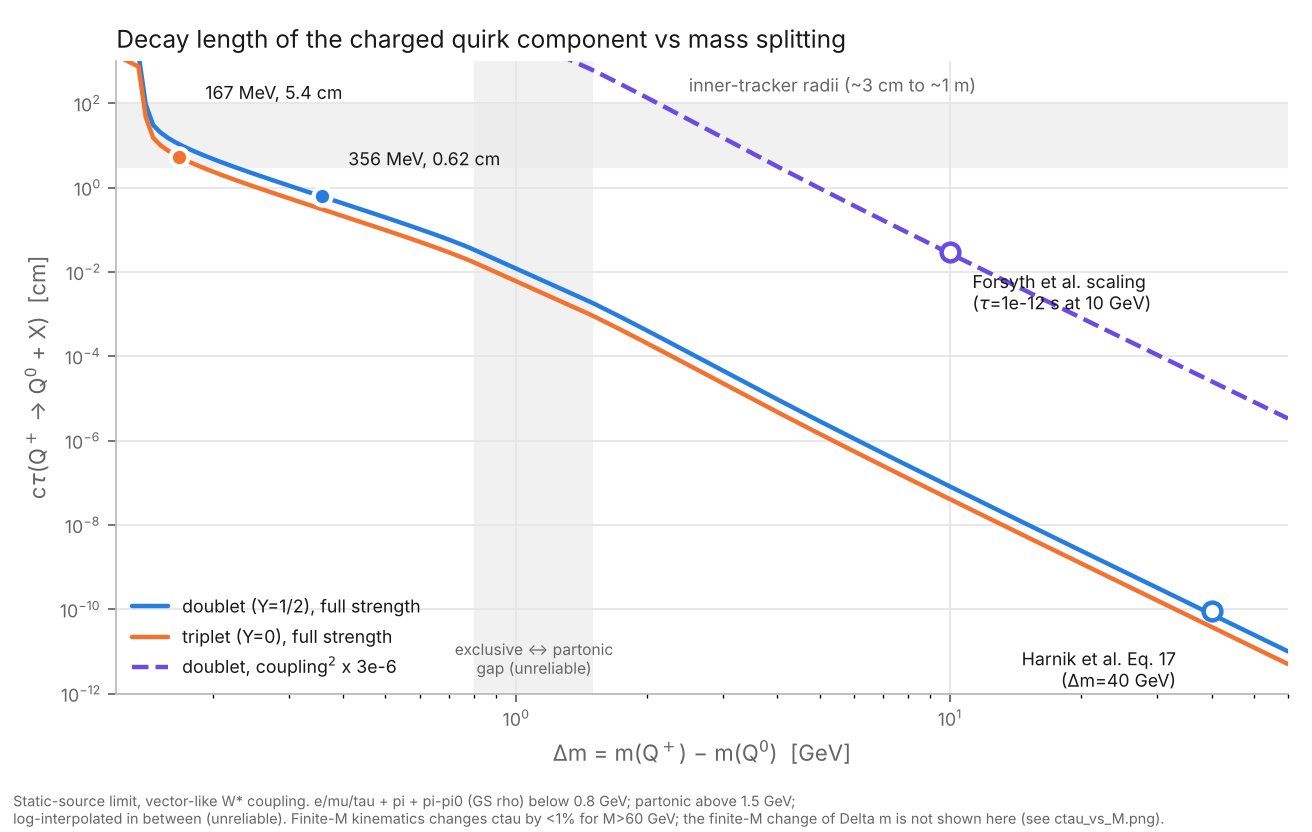
\includegraphics[width=\columnwidth]{figs/ctau_map.png}
\caption{Decay length of $Q^+$ versus $\Delta m$ (one-loop splitting, finite-$M$ kinematics; exclusive $e,\mu,\pi,\pi\pi^0$ channels below $0.8$~GeV, partonic above $1.5$~GeV, interpolated in between with about 20\% uncertainty). TODO: regenerate for the paper style.}
\label{fig:ctau}
\end{figure}

For $M=500$~GeV the doublet has $\Delta m=356$~MeV and $c\tau=6.2$~mm; the triplet has $\Delta m=167$~MeV and, with the $\kappa=2$ of its normalisation, $c\tau=54$~mm, decaying to $\pi^\pm$ in 97.7\% of the cases.

\section{String dynamics with a decay step}
We extend the Geant4 quirk transport of Refs.~\cite{QuirkPheno,Vami:2026} (Apache-2.0, pinned at commit \texttt{d91cb27}) with a discrete process for the charged quirks. The decay length is $\beta\gamma c\tau$, which is memoryless, so re-sampling when a suspended track resumes is exact. At the decay the parent is killed and the neutral quirk and the visible products are created at the same point. The string state of the parent (partner, stored string vectors, last four-velocity) is handed to the neutral daughter, so the partner is not released; only the final end of the daughter frees it. Decay kinematics are generated in the parent rest frame with exact two- and three-body phase space weighted by the squared matrix element (heavy-fermion tensor times lepton tensor for $\ell\nu$; $(k_1-k_2)^\mu(k_1-k_2)^\nu$ for $\pi\pi^0$), because Geant4's generic phase-space decay is numerically unreliable for $M-M_0\ll M$.

Checks (500~GeV, $\Delta m=356$~MeV, 2000 leptonic decays): the proper decay time follows the input exponential (KS $p=0.04$ and $0.40$ for two seeds); four-momentum is conserved to float precision; the rest-frame mean energies are $173$--$181\pm3$~MeV for $e$ and $208\pm2$~MeV for $\mu$ against $177.9$ and $206.8$~MeV from the static-source spectrum. For the triplet (6000 decays) the single-pion momentum in the parent rest frame is $91.686$~MeV against $91.687$~MeV analytic, and the lifetime fit gives $53.6\pm0.7$~mm for an input of $53.9$~mm. The handover is validated in two ways. An identity test (the neutral daughter carrying the parent's identity reproduces the undecayed run) is exact. A field-free vacuum comparison of $300$ pairs at $\Lambda=300$~eV, $c\tau=300$~mm, $\Delta m=2$~MeV against the same kinematics with a neutral quirk from the start agrees in distribution (KS $p\ge0.99$ for the end energy, time, longitudinal position and maximum separation; paired mean differences $\le1.5\sigma$, i.e. $\lesssim3\times10^{-3}$ of the mean) but not event by event (median relative difference $10^{-3}$--$10^{-2}$, with tails). The same per-event spread appears between identity-decay runs whose decay points differ, and between an identity run and a run with no decay, so it comes from the step discretisation of the string integration, which a new decay point changes, and not from the handover.

\section{Regimes in $\Lambda$}
We simulate $13$~TeV Drell--Yan $Q^+Q^-$ pairs at $M=500$~GeV ($|\eta|<2.5$, leading order, NNPDF3.1-LUXqed through Pythia's internal set) in a generic CMS-like detector, for $\Lambda=10$--$3000$~eV and $c\tau=1$--$5000$~mm, with $2000$ charged quirks at each of the $42$ points (Fig.~\ref{fig:maps}); this grid uses the asymptotic $\Delta m$ and the triplet decay table throughout, the mass scan below uses the finite-$M$ splitting and the table of each representation.

\begin{figure*}[t]
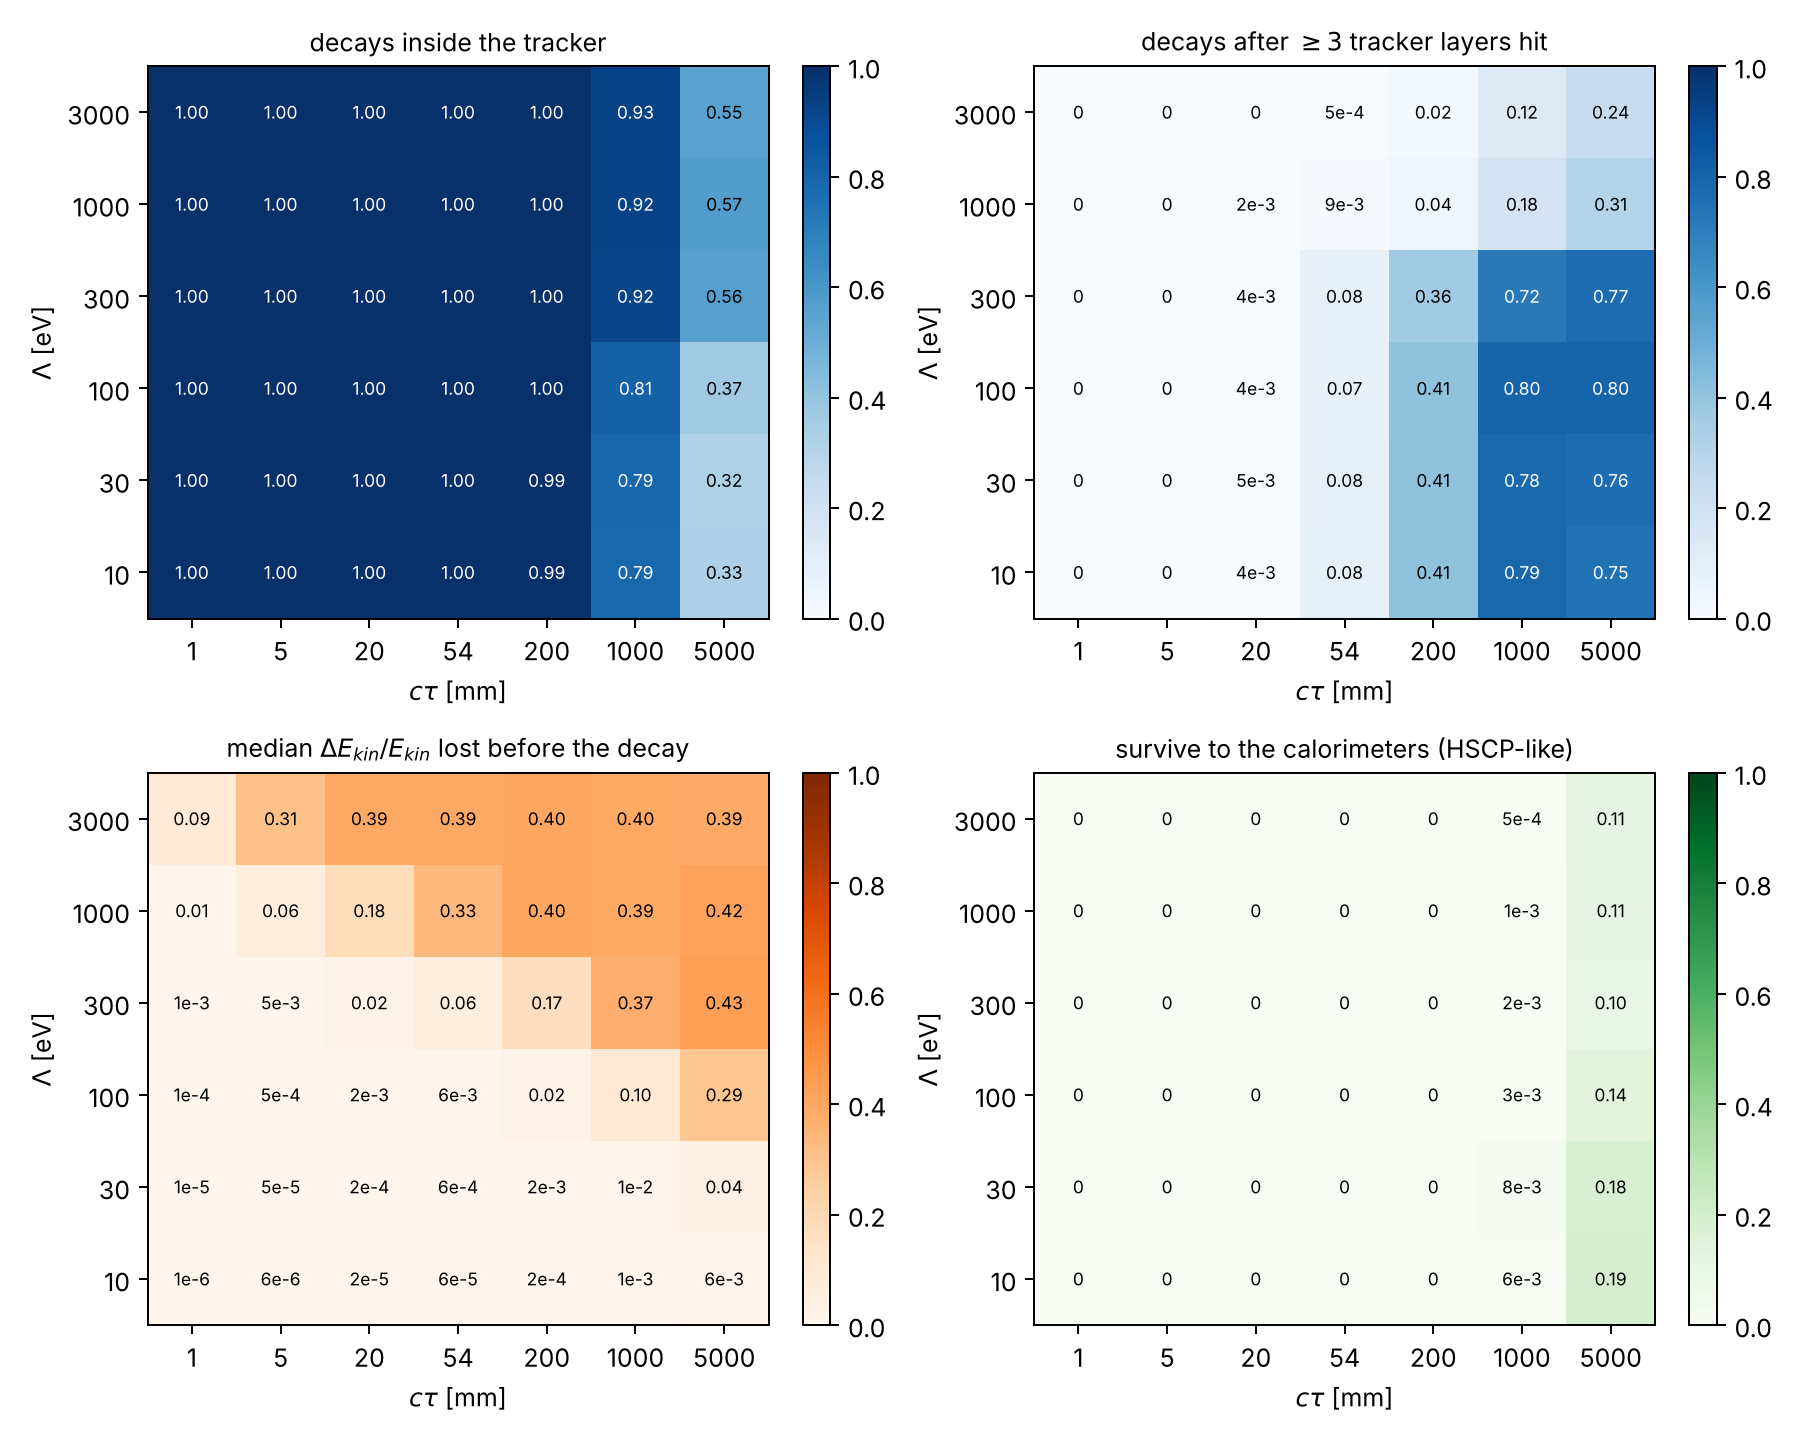
\includegraphics[width=0.8\textwidth]{figs/scan_triplet_M500_maps.png}
\caption{Fractions of charged quirks that decay inside the tracker, decay after leaving hits in at least three tracker layers, median fractional kinetic-energy loss to the string before the decay, and fraction reaching the calorimeters. $M=500$~GeV, triplet decay table throughout the grid.}
\label{fig:maps}
\end{figure*}

\emph{Decay length.} For $c\tau\le 200$~mm essentially all charged quirks decay inside the tracker for any $\Lambda$. At the benchmark lengths the decay occurs before the quirk crosses three layers in nearly every case: for the doublet ($c\tau=6.2$~mm) $0.05\%$ leave hits in three or more layers and the mean number of layers hit is $0.01$; for the triplet ($c\tau=54$~mm) the numbers are $7$--$9\%$ and $0.7$ for $\Lambda\le 300$~eV. The charged leg therefore terminates inside or before the pixel detector; a reconstructed terminating track needs $c\tau\gtrsim 0.2$~m ($41\%$ with at least three layers) and about $80\%$ ($\Lambda\le100$~eV; $72\%$ at $300$~eV) are reached at $c\tau=1$~m. This is a statement about hits recorded by the simulation, not about track-reconstruction efficiency.

\emph{String energy loss.} Below saturation the kinetic energy lost to the string before the decay follows $\Delta E\simeq 0.72\,T L_d$ with $T=\Lambda^2/\hbar c$ and $L_d$ the median decay distance (Fig.~\ref{fig:loss}; the ratio has median $0.72$ and range $0.65$--$1.2$ over the $27$ grid points with $\Delta E<0.1\,E_{\rm kin}$). The loss saturates at about $90$~GeV, a third of the median kinetic energy of $276$~GeV of this sample. For the triplet benchmark the median fractional loss before the decay is $6\times10^{-5}$, $6\times10^{-3}$, $6\times10^{-2}$ and $0.35$ at $\Lambda=10$, $100$, $300$ and $1000$~eV; for the doublet it is $7\times10^{-6}$, $7\times10^{-4}$, $6\times10^{-3}$ and $0.07$. The loss, and with it the departure of the charged leg from a helix, reaches about $6\%$ for the triplet at $300$~eV; for the doublet it stays below $1\%$ up to $300$~eV.

\begin{figure}[t]
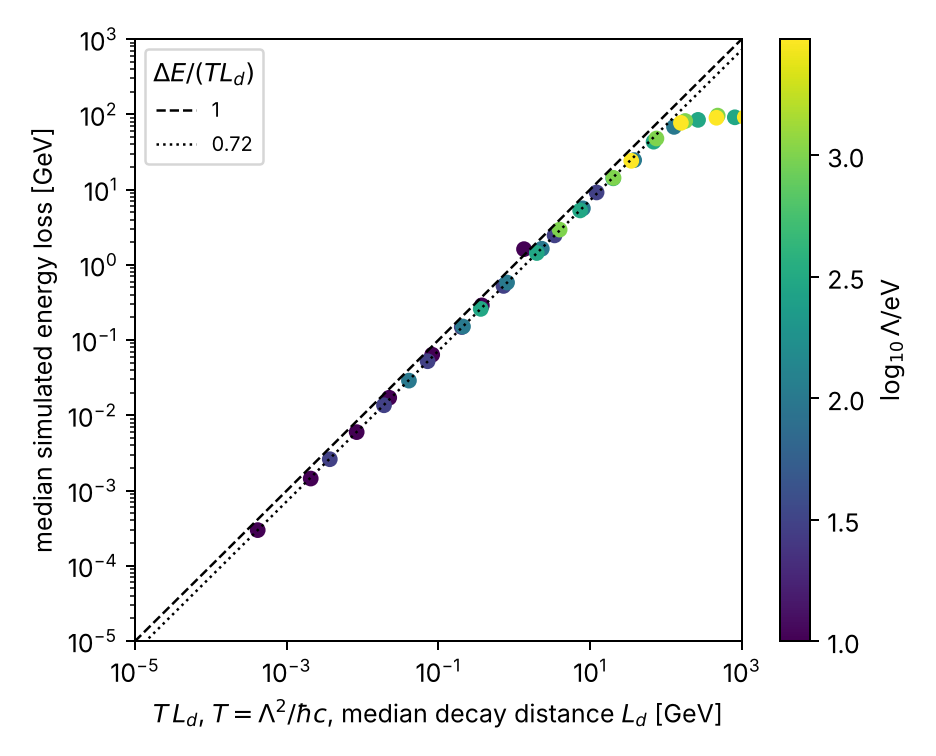
\includegraphics[width=\columnwidth]{figs/scan_triplet_M500_loss_check.png}
\caption{Simulated median energy loss before the decay against $T L_d$ for all scan points with more than half of the quirks decayed.}
\label{fig:loss}
\end{figure}

\emph{Surviving quirks.} Only for $c\tau=5$~m do $10$--$19\%$ of the charged quirks reach the calorimeters, so for the EW-multiplet benchmarks the charged track does not reach the calorimeters and muon system on which the stable-quirk searches of Refs.~\cite{Vami:2026,FASER:2026} rely; quantifying the remaining sensitivity needs the recast of Sec.~\ref{sec:recast}. The neutral partner has only string interactions and the pair of neutral quirks leaves the detector as missing momentum for small $\Lambda$; its string interactions and the merged-pair regime at large $\Lambda$ are not studied here.

\emph{Helical or not.} A reconstruction that fits a helix to the hits accepts the charged leg while the string force is small against the magnetic force. We fit a circle in the transverse plane to the hit mid-points of each charged quirk with at least four tracker hits, with the hits smeared by $10$~$\mu$m (pixel) and $30$~$\mu$m (strip), and call the track helical-compatible if the geometric fit has $\chi^2/{\rm ndf}<3$ and a radius above $0.5$~m; no pattern recognition, material effects or longitudinal fit are included, so this is a proxy for the track-fit acceptance, not a reconstruction efficiency. At $c\tau=1$ ($5$)~m the helical-compatible fraction is $0.97$ ($0.97$--$0.99$) for $\Lambda\le30$~eV (the $\chi^2$ cut alone costs about $8\%$ for four hits), $0.81$ ($0.60$) at $100$~eV, $0.28$ ($0.10$) at $300$~eV and $0.006$ ($0.002$) at $1$~keV (Fig.~\ref{fig:helix}). Without smearing, with a $0.1$~mm RMS cut, the same fractions are $0.92$ ($0.76$), $0.49$ ($0.21$) and $0.27$ ($0.17$) at $100$, $300$ and $1000$~eV, so the unsmeared proxy overestimates the acceptance, strongly so at $1$~keV where the track is not a circle at all. The fraction depends on the track length through the number of hits. Standard helical searches therefore see the charged leg for $\Lambda\lesssim30$~eV; above about $100$--$300$~eV the track is non-helical for most decay lengths of interest.

\begin{figure}[t]
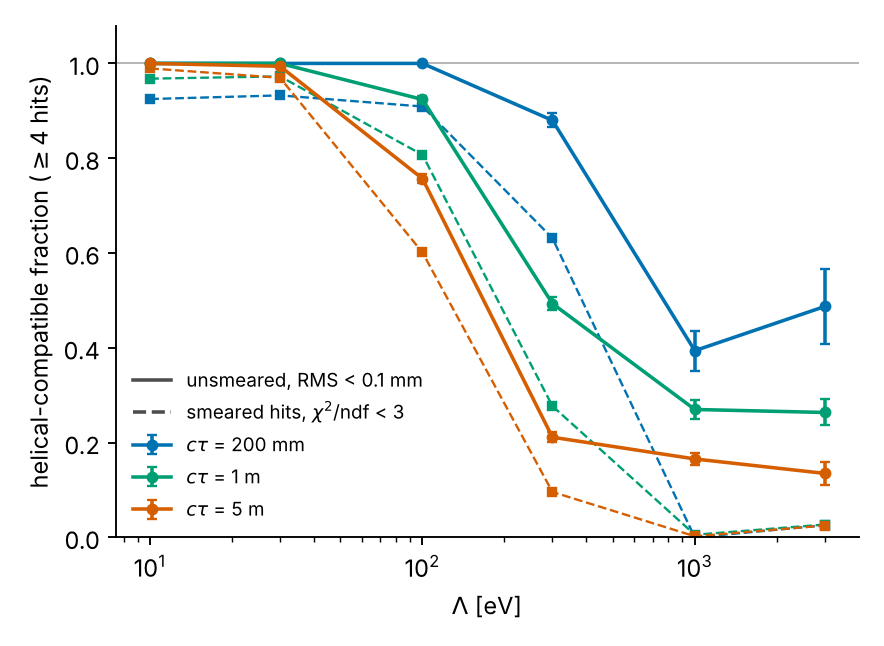
\includegraphics[width=\columnwidth]{figs/helix_fraction_M500.png}
\caption{Fraction of charged-quirk tracks with at least four tracker hits that are helical-compatible, $M=500$~GeV. Solid: RMS of the circle fit below $0.1$~mm on unsmeared hits; dashed: smeared hits, $\chi^2/{\rm ndf}<3$.}
\label{fig:helix}
\end{figure}

\section{Mass dependence and production}\label{sec:mass}
We repeat the scan at $M=300$, $500$, $750$, $1000$, $1500$ and $2000$~GeV with $\Lambda=30$, $100$, $300$ and $1000$~eV, for the doublet ($T=\tfrac12$, $Y=\tfrac12$, $\kappa=1$) and the triplet ($T=1$, $Y=0$, $\kappa=2$) at each mass, with the one-loop splitting at finite $M$ (doublet $\Delta m=314\to349$~MeV and $c\tau=9.5\to6.6$~mm, triplet $\Delta m=164\to167$~MeV and $c\tau=59.5\to54.2$~mm for $M=300\to2000$~GeV) and the decay table computed for each case. Both production modes are simulated: Drell--Yan $Q^+Q^-$ and the $W^*$-mediated $Q^\pm Q^0$ (Pythia process~3021 with an off-shell, vector-like $W'$ at the $W$ mass). Each sample has $2000$ generator events per mode and mass, filtered to $|\eta|<2.5$ for the pair or one quirk, with $2000$ charged quirks per point in the main grid. The Drell--Yan events come from Pythia's $\gamma^*/Z$ with the couplings of a chiral fourth-generation lepton; we re-weight them event by event to the vector-like couplings of the charged member ($\langle w\rangle=1.8$--$2.0$ for the doublet, $6.1$--$7.2$ for the triplet; leading-order formula, massless initial quarks, mass-dependent angular terms approximated). The $W^*$ rate is multiplied by $\kappa_W^2=2$ for the triplet, and the triplet rates by a further factor $2$ for the two charged Dirac species (a Dirac triplet is equivalent to two Majorana winos).

\emph{Production.} The $W^*$ channel dominates over the whole range (Fig.~\ref{fig:xsec}): at $M=500$~GeV the leading-order rates in the filtered region are $5.3$ ($36$)~fb for Drell--Yan and $19$ ($75$)~fb for $W^*$ for the doublet (triplet), at $1$~TeV $0.13$ ($0.85$)~fb and $0.50$ ($2.0$)~fb, at $2$~TeV $5.2\times10^{-4}$ ($3.8\times10^{-3}$)~fb and $3.1\times10^{-3}$ ($1.2\times10^{-2}$)~fb. Without $W^*$ the total rate would be underestimated by a factor $4.5$--$7$ (doublet) and $3.1$--$4.3$ (triplet). The $W^*$ events contain one charged quirk, so the terminating-track yield per event is about half that of Drell--Yan, and the neutral partner is the other end of the string. Two checks fix the normalisation. (i) Pythia's own supersymmetric chargino--neutralino processes with a degenerate pure-wino spectrum, the same PDF set and $13$~TeV give, at $M=500$~GeV, $19.9$~fb for $\chi^+\chi^-$ and $41.2$~fb for $\chi^\pm\chi^0$; the re-weighted Drell--Yan and the $W^*$ total per Majorana wino are $0.96$ and $0.95$ of these ($0.96$, $0.99$ at $300$~GeV; $0.89$, $0.89$ at $1$--$2$~TeV), and the Drell--Yan to $W^*$ ratio $0.48$ agrees with that of the wino processes. (ii) Against the published next-to-leading-order plus next-to-leading-logarithm wino cross section of $3.42$~fb at $850$~GeV (ATLAS three-lepton search~\cite{ATLAS:3l}), the Pythia supersymmetric leading-order value, interpolated in mass, requires $K=1.13$, and my own tables $K\simeq1.25$; this single anchor is assumed to apply at all masses and to both channels, and the tables in this paper are not rescaled.

\begin{figure}[t]
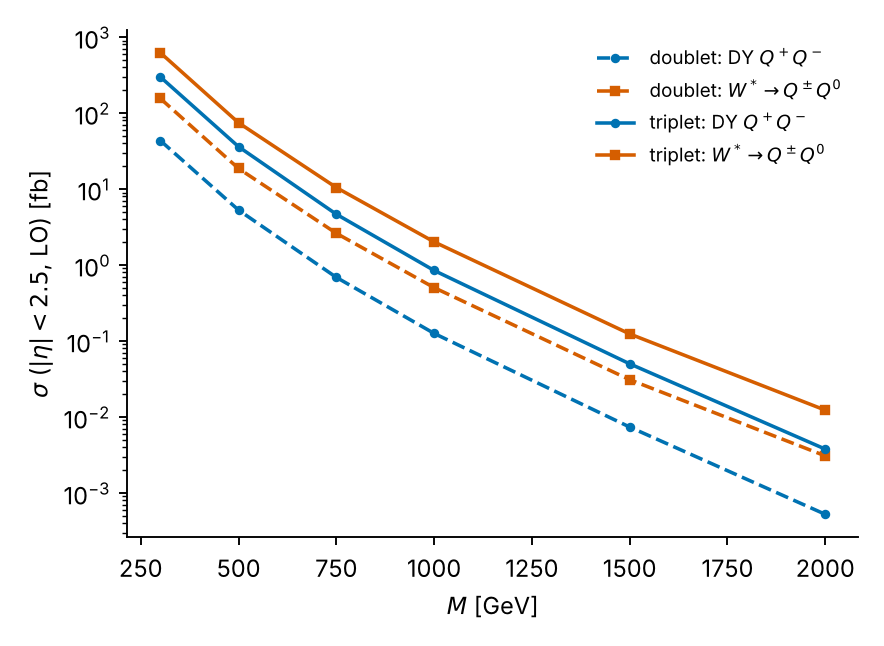
\includegraphics[width=\columnwidth]{figs/massscan_xsec.png}
\caption{Leading-order production cross sections ($|\eta|<2.5$ filter) against the quirk mass.}
\label{fig:xsec}
\end{figure}

\emph{Terminating tracks.} For the triplet the number of charged-quirk decays inside the tracker after hits in at least three layers is, before any reconstruction efficiency, $123$, $13$, $1.0$, $0.13$, $6.0\times10^{-3}$ and $5.1\times10^{-4}$~fb at $M=300$, $500$, $750$, $1000$, $1500$ and $2000$~GeV for $\Lambda=100$~eV (Fig.~\ref{fig:yield}, left), that is $4\times10^4$ events at $3$~ab$^{-1}$ for $M=500$~GeV, $\sim380$ at $1$~TeV and $\sim18$ at $1.5$~TeV; it is the same within $20\%$ for $\Lambda\le300$~eV and a factor $8$--$20$ lower at $1$~keV for $M=300$--$1000$~GeV, where the energy loss to the string takes the quirk away from the sensitive layers before three are crossed. For the doublet the decay is too short: $0.39$~fb at $M=300$~GeV, $4\times10^{-3}$~fb at $500$~GeV and no event above.

\emph{Neutral-pair signature.} After the decay the pair is neutral. We classify the event as a neutral pair leaving the detector if a charged quirk decayed and both quirks end by leaving the detector volume (or because the partner did); the missing momentum is estimated by the generator-level transverse momentum of the pair, as the decay products are soft. Over the whole grid $90$--$99.8\%$ of the events end this way ($97$--$99.8\%$ at $\Lambda=30$~eV, $90$--$98\%$ above), and $0.2$--$10\%$ (larger for larger $M$ and $\Lambda$) still have a quirk alive at the $500$~ns limit, as expected for a bound pair that oscillates and is not leaving. Every event with $p_T^{\rm pair}>250$~GeV leaves, so the yield above this threshold is independent of $\Lambda$ and falls from $6.8$ ($1.5$)~fb at $500$~GeV to $0.22$ ($0.048$)~fb at $1$~TeV and $2.3\times10^{-3}$ ($5.2\times10^{-4}$)~fb at $2$~TeV for the triplet (doublet) (Fig.~\ref{fig:yield}, right). A monojet-style selection at generator level (anti-$k_T$ $R=0.4$ jets from the visible final-state particles, leading jet $p_T>100$~GeV and $|\eta|<2.4$, missing momentum from the visible particles above $250$~GeV, no $\Delta\phi$, jet-multiplicity or lepton requirement, trigger efficiency taken as unity) keeps $41$, $6.3$, $1.2$, $0.22$, $0.021$ and $0.0022$~fb for the triplet at $M=300$--$2000$~GeV ($8.9$, $1.3$, $0.27$, $0.048$, $4.7\times10^{-3}$, $5\times10^{-4}$~fb for the doublet); with the threshold at $400$~GeV the triplet yields are $13$, $2.2$, $0.48$ and $0.092$~fb at $300$--$1000$~GeV. For scale, the ATLAS $139$~fb$^{-1}$ monojet model-independent limit quoted in Ref.~\cite{Tumblers:2021} is $\sigma\times A\times\epsilon<736$~fb for a recoil above $200$~GeV (we have not re-checked it against the ATLAS paper), so the neutral pair alone is not constrained by monojet searches at these masses. There is no detector simulation of jets or missing momentum.

\begin{figure*}[t]
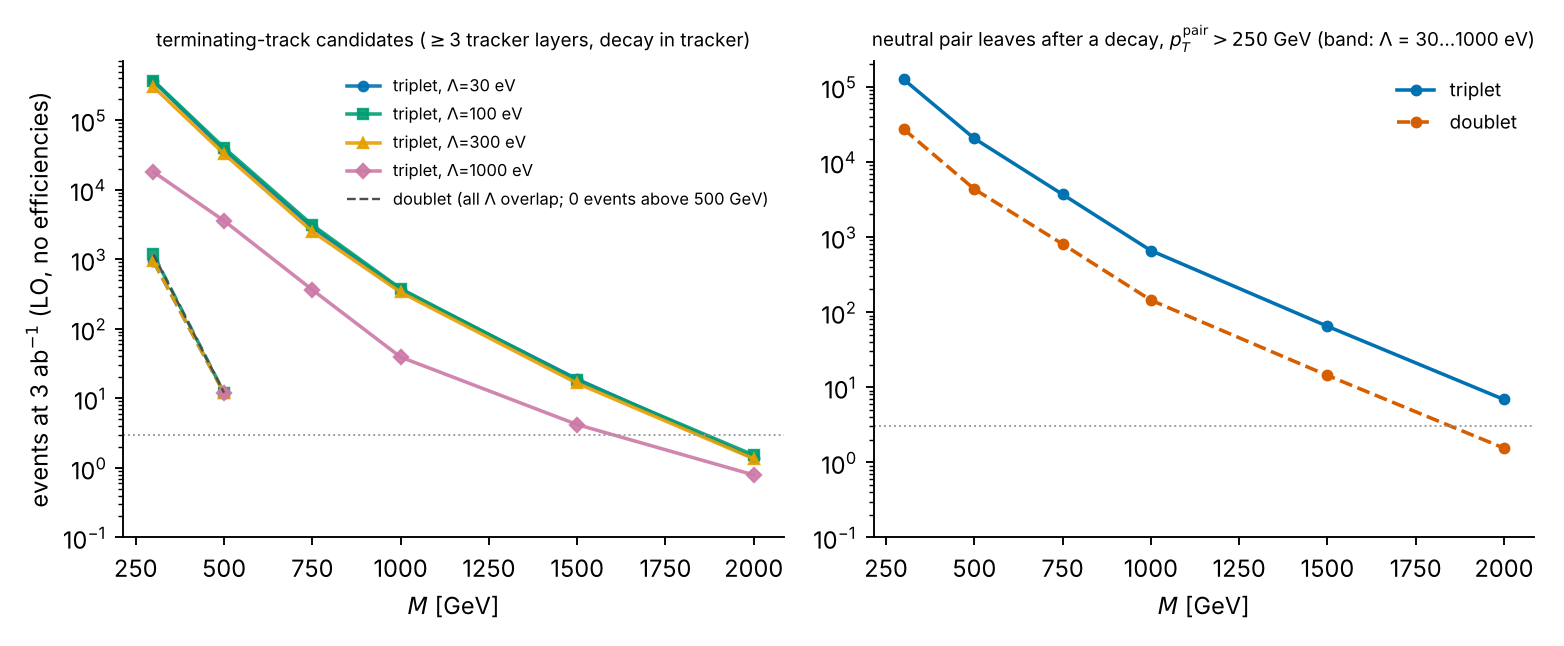
\includegraphics[width=0.95\textwidth]{figs/massscan_yield.png}
\caption{Events at $3$~ab$^{-1}$ (leading order, no efficiencies). Left: charged quirk decays in the tracker after hits in at least three layers, triplet for $\Lambda=30$--$1000$~eV and doublet (all $\Lambda$ overlap). Right: neutral pair leaves the detector after a charged-quirk decay with $p_T^{\rm pair}>250$~GeV; the bands span $\Lambda=30$--$1000$~eV.}
\label{fig:yield}
\end{figure*}

\emph{Sensitivity checks.} (i) Replacing the decay products of the triplet by those of the doublet table at the same $c\tau$ and $\Delta m$ changes the terminating-track fractions by at most $4\%$ ($0.177\to0.178$ at $\Lambda=100$~eV), so the table affects the visible products but not these quirk-based observables. (ii) An ITk-like layout, with five pixel and four strip barrel layers at radii typed from memory of the public layout (not verified against the technical design reports) and $B=2$~T, gives a terminating-track fraction lower by a factor $2$ for $\Lambda\le300$~eV ($0.177\to0.085$ for Drell--Yan, $0.101\to0.044$ for $W^*$ at $100$~eV) and by a factor $3$--$12$ at $1$~keV, while the neutral-pair yield is unchanged. The detector dependence is therefore at least a factor two, and the numbers above should be read as CMS-like.

\emph{Limits.} Leading order, no electroweak corrections; $W^*$ and Drell--Yan are generated with the $W'$ and $\gamma^*/Z$ templates of Pythia and re-weighted analytically (agreement with Pythia's wino processes within $4$--$11\%$); one sample of $2000$ events per point with the statistical precision of the fractions of a few per cent at $M=500$~GeV and worse at high $M$ where few quirks have four hits; sensitive-volume hits rather than reconstructed tracks; two generic detector layouts; $\Lambda>3$~keV not studied. A forced step in the transport that leaves the world was found to crash events at small $\Lambda$ and is handled by killing the quirk (see the code repository).

\section{Recasts of public searches}\label{sec:recast}
\emph{Track-based HSCP searches.} These require the charged quirk to reach the outer tracker or the muon system. Using the generator kinematics of the mass-scan samples, the probability that at least one charged quirk reaches the end of the tracker before decaying is $8.8\times10^{-5}$, $7.5\times10^{-6}$, $5.7\times10^{-7}$, $9.1\times10^{-8}$, $3.8\times10^{-8}$ and $2.1\times10^{-8}$ for the triplet at $M=300$, $500$, $750$, $1000$, $1500$ and $2000$~GeV (straight-line path, no string slowing or bending, so these are upper estimates; the median string loss before the decay is below $1\%$ for $\Lambda\le100$~eV and $6\%$ at $300$~eV for the triplet), and below $10^{-15}$ for the doublet; the muon-system probabilities are smaller by a further $3.5$--$5$ orders of magnitude. The surviving triplet cross section is $0.081$~fb at $300$~GeV, $8.3\times10^{-4}$~fb at $500$~GeV and below $10^{-5}$~fb from $750$~GeV, and zero for the doublet. The most sensitive published limit of this type that we use, the CMS ionization search~\cite{CMS:2024HSCP} (Drell--Yan $\tau'$ with $Q=1e$ excluded below $1.02$~TeV with $101$~fb$^{-1}$), has a high-mass plateau of $0.066$~fb in the flat-limit approximation (derived from the quoted mass reach and our own cross section of the $\tau'$-like pair); with this optimistic plateau, the HSCP search does not exclude the benchmark spectra. The survival probability reaches $0.27$ ($0.16$) at $c\tau=1$~m for $M=500$ ($1000$)~GeV and $0.76$ ($0.67$) at $5$~m, so the HSCP recast applies to spectra with $c\tau\gtrsim1$~m, which for the triplet means $\Delta m\lesssim0.13$~GeV, below the charged-pion threshold, and is not the gauge-loop splitting of Sec.~\ref{sec:mass} ($\Delta m=0.164$--$0.167$~GeV); it needs an additional contribution to the splitting. For such a spectrum the same flat-limit comparison gives surviving triplet cross sections of $0.45$ ($1.9$)~fb at $M=1$~TeV and $0.020$ ($0.11$)~fb at $1.5$~TeV for $c\tau=1$ ($5$)~m, that is exclusion to about $1.3$ ($1.6$)~TeV, an optimistic estimate because the plateau is the strongest limit of the search, the string slowing is neglected and the search efficiency for a quirk with a neutral partner at the end of a string is not simulated. We have not used the published limit curves, whose tabulated values we could not retrieve in this environment.

\emph{Disappearing-track searches.} For $\Lambda\lesssim30$~eV the charged leg is helical and the signature is that of a disappearing track with a decay length of $5.4$~cm and a pion that is lost, the case of a Dirac triplet (twice the production of the Majorana wino at the same mass). We calibrate on the published wino exclusions and use a flat-limit approximation: a mass is excluded if the triplet cross section times the terminating-track efficiency relative to its $\Lambda=30$~eV value equals the wino-equivalent cross section (half the triplet) at the calibration mass; with our own leading-order cross sections on both sides, the $K$-factor cancels. Calibrating on the ATLAS wino exclusion of $660$~GeV at $0.2$~ns~\cite{ATLAS:DT}, the Dirac triplet ($c\tau=54$--$59$~mm) is excluded to $754$, $764$ and $734$~GeV at $\Lambda=30$, $100$ and $300$~eV; calibrating on the CMS value of $474$~GeV at $0.2$~ns~\cite{CMS:DT} gives $550$, $559$ and $535$~GeV. At $1$~keV the relative efficiency is about $0.03$, which is outside the range where the calibration means anything, and the track is not helical, so we claim no sensitivity there. The numbers are uncertain by about $\pm15$~GeV from the Monte Carlo statistics alone and, more importantly, ignore the mass dependence of the published efficiency and limit and the track-quality requirements: with the smeared helix fraction above ($0.81$ at $100$~eV, $0.28$ at $300$~eV for $c\tau=1$~m) the effective efficiency of a standard disappearing-track reconstruction is lower for $\Lambda\gtrsim100$~eV. The doublet ($c\tau\approx7$--$10$~mm) decays within the pixel detector and has no exclusion.


\section{The turnaround window}
TODO: terminating coplanar-hit selection.

\section{Conclusions}
TODO.

\begin{acknowledgments}
TODO.
\end{acknowledgments}

\bibliographystyle{apsrev4-2}
\bibliography{refs}

\end{document}
